%%
% Please see https://bitbucket.org/rivanvx/beamer/wiki/Home for obtaining beamer.
%%
%\documentclass[11pt,aspectratio=169]{beamer}
%\documentclass[11pt,aspectratio=169,xcolor={dvipsnames}]{beamer}

\documentclass[11pt,aspectratio=169,xcolor={dvipsnames},hyperref={pdftex,pdfpagemode=UseNone,hidelinks,pdfdisplaydoctitle=true},usepdftitle=false]{beamer}
\usepackage{presentation}


\title{Lecture 7: Government Expenditure Multiplier}
\author{Juan Herre\~{n}o\\UCSD}
\date{2026}

% Enter presentation title to populate PDF metadata:
\newcommand{\Cov}{\text{Cov}_\lambda}
\newcommand{\El}{\mathbb{E}_\lambda}
\newcommand{\mm}{\text{{\fontfamily{qzc}\selectfont m}}}
\usepackage{cancel}
\begin{document}

\maketitle


\begin{frame}{Of Multipliers and Parameters}
\begin{itemize}
\item Macroeconomists are often interested in two types of objects
\begin{itemize}
\item Invariant structural parameters. Usually they are primitives related to preferences, or technologies. They are invariant to shocks.
\item Elasticities: functions of parameters, prices, equilibrium outcomes
\end{itemize}
\item Caveat: Complicate models: structural parameter $\rightarrow$ elasticities
\item Caveat II: Simplify models: elasticities $\rightarrow$ structural parameter
\end{itemize}
\end{frame}


\begin{frame}{Of Multipliers and Parameters}
\begin{itemize}
\item In our models the multiplier is \textbf{not} a structural parameter
\item Implications of that: In principle
\begin{itemize}
\item Depends on policy regimes (lean against the wind)
\item Depends on how it is financed (taxes vs. transfers from abroad)
\item Depends on the real interest rate (crowding out)
\item Depends on the underlying structure of the economy (is there capital? is the economy open?)
\end{itemize}
\item There is not \textbf{ONE} multiplier
\item Also, notice that households do not care about output in itself; they care about consumption and leisure. It is not obvious that more production is good for welfare.
\end{itemize}
\end{frame}


\begin{frame}{Multipliers in the Neoclassical Model}
\begin{itemize}
\item Suppose
$$\max_{C_t,H_t} \sum_{t=0}^{\infty} \beta^t \left[u(C_t) - v(H_t) + \Gamma(G_t)\right]$$
\vspace{-0.5cm}
$$Y = f(H_t)$$
\vspace{-0.5cm}
$$Y_t = C_t + G_t$$
\vspace{-0.5cm}
\item All prices flexible. All markets competitive
\item No capital. No durables. No assets in net supply
\item The government picks $G$ (not the household!)
\item Taxation in lump-sum taxes
\item What is the effect of increases in $G_t$ on $Y_t$
\end{itemize}
\end{frame}



\begin{frame}{Multipliers in the Neoclassical Model}
Intratemporal optimization yields
$$\frac{v'(H_t)}{u'(C_t)} = \frac{W_t}{P_t}$$
Profit maximization yields
$$f'(H_t) = \frac{W_t}{P_t}$$
Combined yield
$$\frac{v'(H_t)}{u'(C_t)}  = f'(H_t)$$
\end{frame}


\begin{frame}{Multipliers in the Neoclassical Model}
Rearrange
$$\frac{v'(H_t)}{ f'(H_t)}  = u'(C_t)$$
\begin{itemize}
\item RHS: marginal utility of consumption
\item LHS: Marginal disutility of producing output.
\end{itemize}
\vspace{1cm}
Use the production function and the resource constraint $Y = C + G$ And the production function $Y = f(H)$
$$ u'(Y_t - G_t) = \tilde{v}'(Y_t) $$
\end{frame}


\begin{frame}{Multipliers in the Neoclassical Model}
$$ u'(Y_t - G_t) = \tilde{v}'(Y_t) $$
Then the multiplier $\frac{dY}{dG}$ is given by
$$\frac{dY}{dG} = \frac{\eta_u}{\eta_u + \eta_{\tilde{v}}}$$
Where
\begin{itemize}
\item $\eta_u > 0$ is the negative of the elasticity of $u'$ ($-\bar{Y}u''/u'$)
\item $\eta_{\tilde{v}} > 0$ is the elasticity of $\tilde{v}'$ ($\bar{Y}\tilde{v}''/\tilde{v}'$)
\end{itemize}
That is, the multiplier is between zero and one.
\end{frame}

\begin{frame}{Multipliers in the Neoclassical Model}
$$\frac{dY}{dG} = \frac{\eta_u}{\eta_u + \eta_{\tilde{v}}}$$
\begin{itemize}
\item Multiplier between zero and one
\item Government spending ``crowds-out'' private spending
\item Government consumes some stuff
\item Households are poorer. Negative wealth effects.
\item Consume less normal goods (leisure and consumption), so work (and produce) more!
\item Multiplier is small iff
\begin{itemize}
\item There is more crowding out
\item Disutility of producing more output rises fast
\item Households have large elasticity of intertemporal substitution
\end{itemize}
\end{itemize}
\end{frame}

\begin{frame}{Multipliers in the Neoclassical Model}
\begin{itemize}
\item Suppose $G$ is temporarily high today. What happens to the real rate?
$$u'(C_t) = \beta R_t u'(C_{t+1})$$
\item There is crowding out, $R_t$ must be high today. (notional interest rate).
\item Notional interest rate. The interest rate that maintains assets in zero net supply and induces the observed path of consumption
\end{itemize}
\end{frame}

\begin{frame}{Multipliers in the Neoclassical Model}
\begin{itemize}
\item No mention of whether taxes occur today or the future
\item It does not show up in any first order condition.
\item Irrelevant. Ricardian equivalence
\item Depends on lots of assumptions, including lump-sum taxes.
\item What it says:
Variation in the timing of lump-sum taxes is irrelevant
\item What it does not say:
Government spending does not matter for output. Obviously it does! $dY/dG > 0$.

\textit{Please remember that. The whole department and the profession are counting on you, and I will be judged by my colleagues if you forget.}
\end{itemize}
\end{frame}


\begin{frame}{Multipliers in the Neoclassical Model}
\begin{itemize}
\item Same environment. News in period $t$ about $G_{t+1}$. No change in $G_t$
\item What is the reaction of $Y_t$?
\pause
\item Nothing. There is no link between periods.
\item Household knows it will be poorer tomorrow. Nothing it can do about it
\item Think of Robinson Crusoe. Output will increase tomorrow of course.
\end{itemize}
\end{frame}

\begin{frame}{Multipliers in the Neoclassical Model}
\begin{itemize}
\item Shock to $G_t$ but in a world with capital accumulation
\item Multiplier smaller or larger?
\pause
\item Smaller. You have more margins to adjust. $C$, $I$, $N$
\item In our models the solution is to adjust all of them by less
\end{itemize}
\end{frame}

\begin{frame}{Multipliers in the Neoclassical Model}
\begin{itemize}
\item Same environment with capital. No $G_t$ but news about $G_{t+1}$.
\item What happens to $Y_t$?
\pause
\item In $t+1$ will work more. That raises $MPK_{t+1}$.
\item Therefore invest in $t$ so that $K_{t+1}$ is higher
\item Higher effect on $Y_t$
\end{itemize}
\end{frame}



\begin{frame}{Does it matter what the government does with the G?}
Two options
\begin{itemize}
\item  Throws the goods in the ocean (or buys tanks and blows them up in some foreign country)
\item Provides services that households would have bought in the marketplace (childcare, daycare, transportation, education)
\end{itemize}
When is the multiplier higher?
\end{frame}


\begin{frame}{Does it matter what the government does with the G?}
\begin{itemize}
\item Multiplier higher if the government engages in ``wasteful'' spending
\item It's all about wealth effects in this model
\item Buys tanks
$u(C_t) - v(H_t) + \Gamma(G_t)$. Higher $G$ reduces $C$, increases $u'$, raising $H$.
\item Alternative extreme assumption.
$u(C_t + G_t)$. Reallocations of $C_t$ vs $G_t$ do not change $u'$. So $H_t$ does not change.
\end{itemize}
\end{frame}


\begin{frame}{Multipliers in the NK Model}
\begin{itemize}
\item Let's move to the NK model
\item No capital. Sticky prices. Flexible wages
\item Firms set prices. Commit to meet demand
$$f'(H_t) \neq \frac{W_t}{P_t}$$
\item Then what determines labor demand?
\pause
\item Product demand!
\item Pump up wages to hire more workers since households \textbf{are} on their labor supply schedule
\end{itemize}
\end{frame}




\begin{frame}{Multipliers in the NK Model}
Mechanics of the NK model multipliers
\begin{itemize}
\item Total demand must hold $Y_t = C_t + G_t$
\item $G_t$ is exogenous
\item Dynamics of $Y$ depend on the dynamics of $C$.
\item What determines $C$?
$$u'(C_t) = \beta R_t u'(C_{t+1})$$
\item Key variable: the real interest rate
\end{itemize}
\end{frame}


\begin{frame}{Multipliers in the NK Model}
$$u'(C_t) = \beta R_t u'(C_{t+1})$$
\begin{itemize}
\item What determines the real interest rate?
\pause
\item Monetary policy and price setting behavior (due to inflation expectations and the Fisher equation)
\item The response of monetary policy is a crucial determinant of NK multiplier	
\item Imagine a policy in which the central bank implements $R_t = R$
\item Then $C_t = C_{t+1}$. So $\frac{dY}{dG} = 1$ because $\frac{dC}{dG} = 0$
\end{itemize}
\end{frame}


\begin{frame}{Multipliers in the NK Model}
$$u'(C_t) = \beta R_t u'(C_{t+1})$$
Imagine now a Taylor rule
\begin{itemize}
\item Fiscal stimulus is inflationary (someone tells me why)
\item Interest rates go up
\item Consumption today goes down
\item Multiplier is less than one
\end{itemize}
Notice that the NK model has no trouble predicting $dC/dG < 0$ and $dY/dG < 1$.
\end{frame}

\begin{frame}{Multipliers in the NK Model}
\begin{itemize}
\item What happens if $i_t = 0$ (the Zero Lower Bound)
\item $G$ is just as Inflationary
\item Nominal interest rates do not react
\item real rates \textbf{decrease}
\item $\frac{dC}{dG} > 0$. so $\frac{dY}{dG} > 1$
\end{itemize}
\end{frame}

\begin{frame}{Main messages}
\begin{itemize}
\item Can have multipliers of the same magnitude in both models.
\item Monetary policy reaction function is key in the NK model
\item The mechanisms are crucially different though
\begin{itemize}
\item In the neoclassical model, all about wealth effects
\item In the NK model, demand determination, price stickiness, and central bank reaction functions are crucial.
\end{itemize}
\end{itemize}
\end{frame}


\begin{frame}{Evidence on the $G$ multiplier}
Several approaches
\begin{itemize}
\item VARs (Blanchard Perotti '02, Gali et al. '07, Perotti '07)
\item Wars as natural experiments (Hall '09, Ramey '11, Barro Redlick '11)
\item Regional Shocks (Nakamura Steinsson '14, Chodorow-Reich '19)
\end{itemize}
\end{frame}

\begin{frame}{Blanchard Perotti '02}
\begin{itemize}
\item Pioneered VARs based estimation for fiscal stimulus:
$$X_t = A(L)X_{t-1} + U_t$$
\item where $X_t = [T_t, G_t, Y_t]$
\item Four lags
\item Various detrending methods plus dummy variables for seasonality
\item Data from 1960:1-1997:4 (No Korean War)
\end{itemize}
\end{frame}

\begin{frame}{Blanchard Perotti '02}
\begin{itemize}
\item They argue:
\begin{itemize}
\item VARs better suited to understand fiscal stimulus than monetary policy
\item Reason. Implementation lags imply no response of $G$ to $Y$ within a period (effectively, a quarter).
\end{itemize}
\item Identifying assumption is framed as contemporaneous correlation between $G_t$ and $Y_t$ goes from $G_t$ to $Y_t$, not from $Y_t$ to $G_t$
\item If that's the only assumption, why don't we just run
$$Y_{t} = \alpha + \beta G_t + \epsilon_{t} ?$$
\item Because that's not the only assumption! Bigger concern is OVB
\item Something that affects $Y_{t}$ (so goes into $\epsilon_{t}$) correlates with $G_t$
\item VAR assumption is that $A(L)X_t$ control for all those things. Really?
\end{itemize}
\end{frame}

\begin{frame}{Ramey 2011}
Narrative approach
\begin{itemize}
\item Identify shocks to government spending
\item Idea: Business Week forecasted large increases in defense spending
\item Main episodes: Korean War (1950Q3), Vietnam War (1965Q1), Carter-Reagan buildup (1980Q1), 9/11 (2001Q3)
\end{itemize}
Great paper with a great title: ``it's all about the timing''
\begin{itemize}
\item News dates precede increases in $G$, so $G$ shocks are anticipated! 
\item Recall our theoretical discussion. With capital, news about future $G_{t+1}$ increase $H_{t}$, and decrease $C_{t}$. If you start measuring in $t+1$, you miss those effects.
\end{itemize}
\end{frame}

	
\begin{frame}{Why Wars?}
\begin{figure}
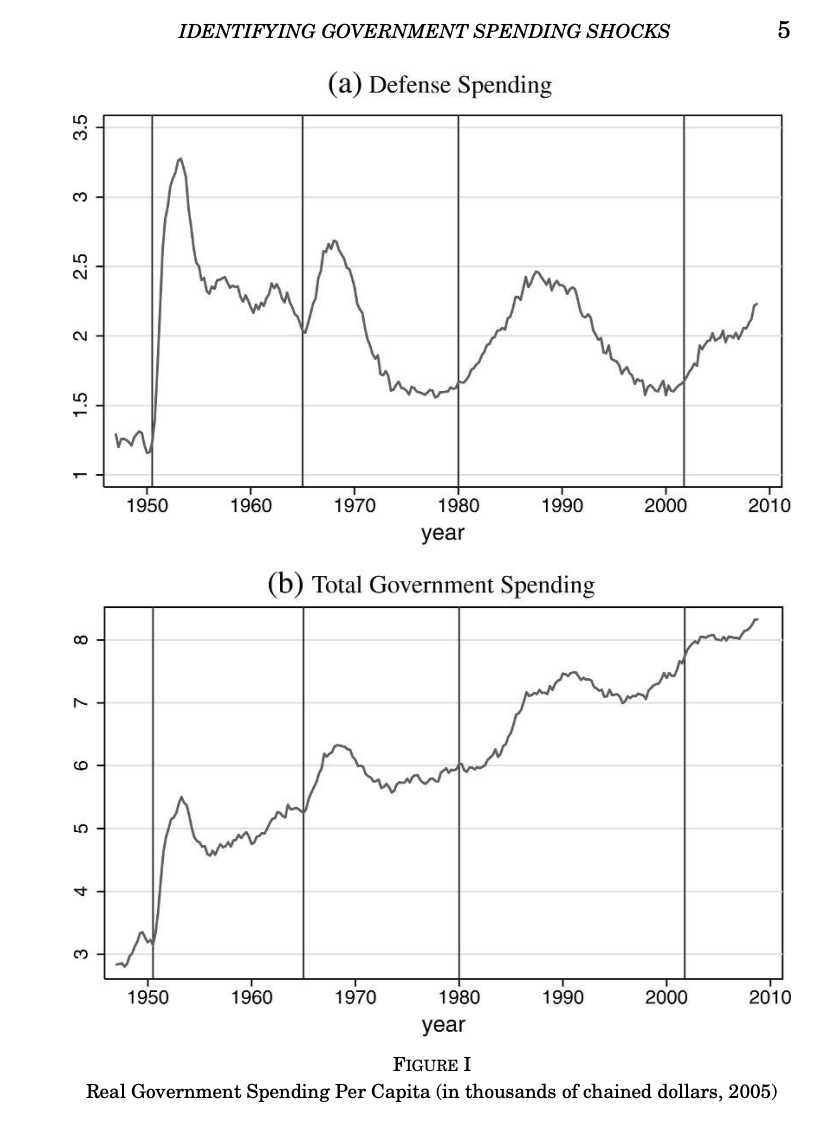
\includegraphics[scale=0.35]{FiguresTables/ramey_1}
\end{figure}
\end{frame}

\begin{frame}{Why Wars?}
\begin{figure}
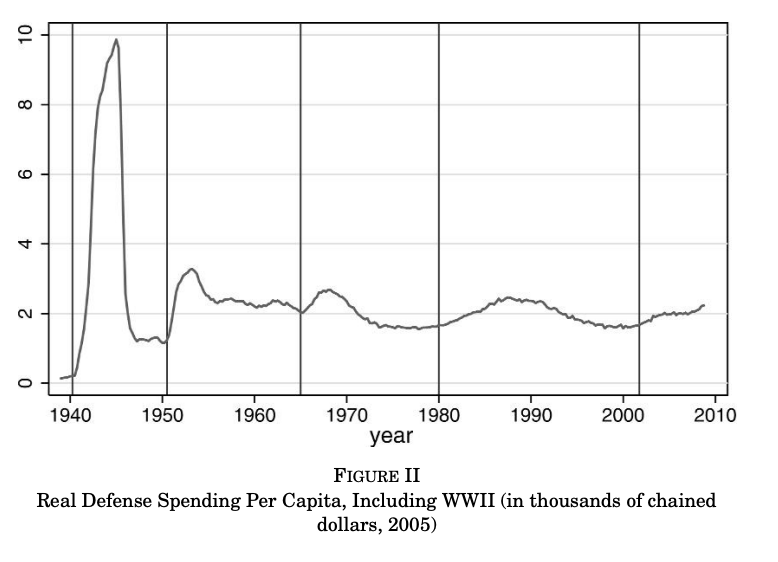
\includegraphics[scale=0.7]{FiguresTables/ramey_2}
\end{figure}
\end{frame}


\begin{frame}{VAR Shocks vs. War Dates}
\begin{figure}
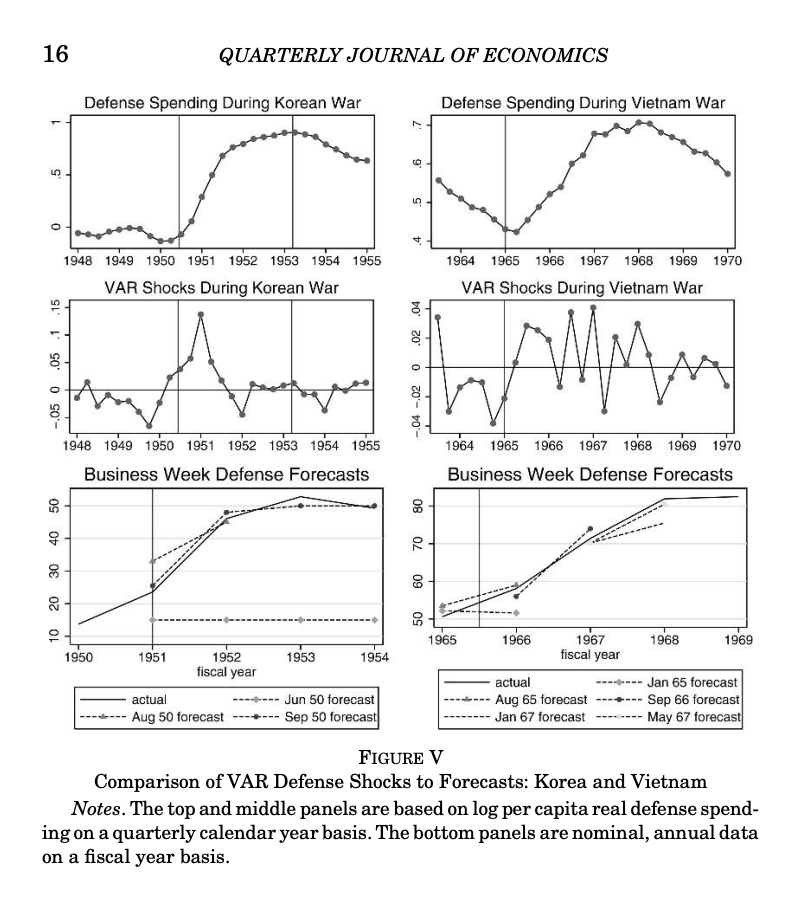
\includegraphics[scale=0.5]{FiguresTables/ramey_3}
\end{figure}
\end{frame}

\begin{frame}{Research Design}
\begin{itemize}
\item Use the War Dates as shocks
\item Use a VAR to compute the Impulse Response Functions
\item VAR with: War Dates, G, Y, H, C, I, $\tau$, W/P
\item Quadratic trends, four lags
\item Sample period: 1947-2008
\end{itemize}
\end{frame}

\begin{frame}{IRFs}
\begin{figure}
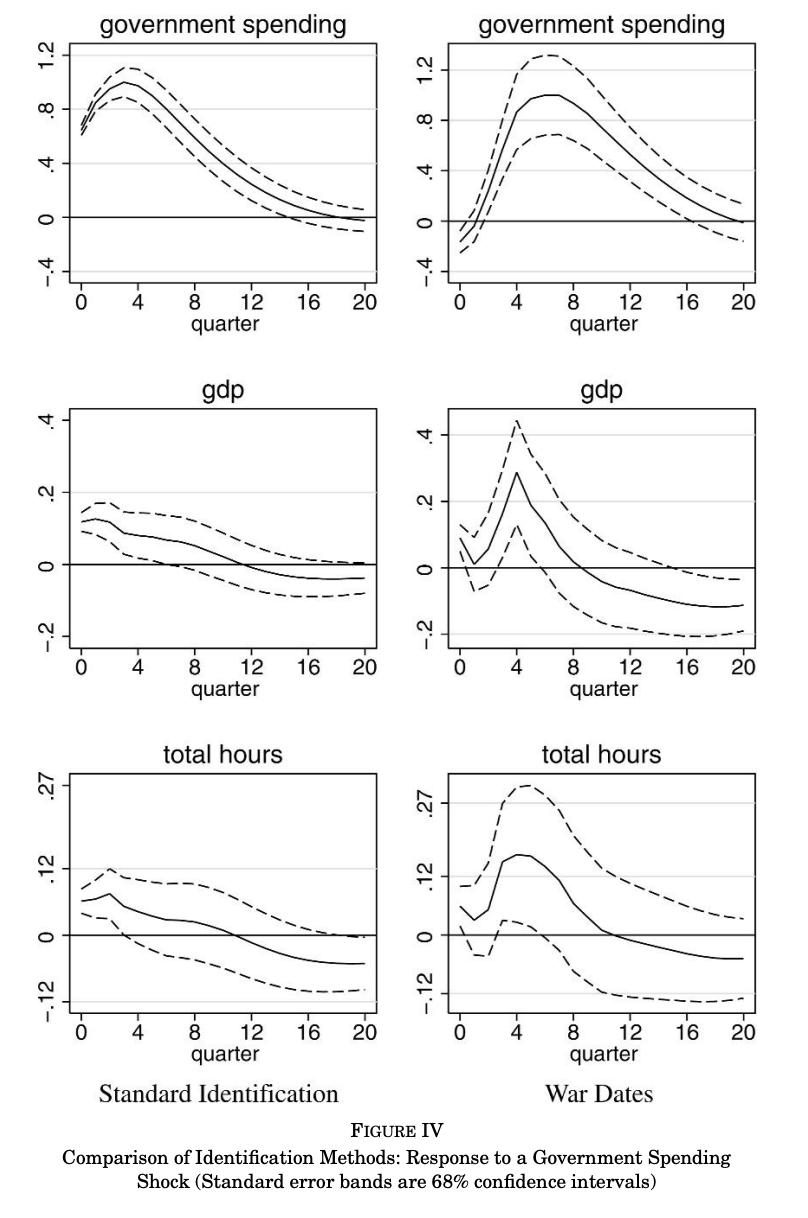
\includegraphics[scale=0.35]{FiguresTables/ramey_4}
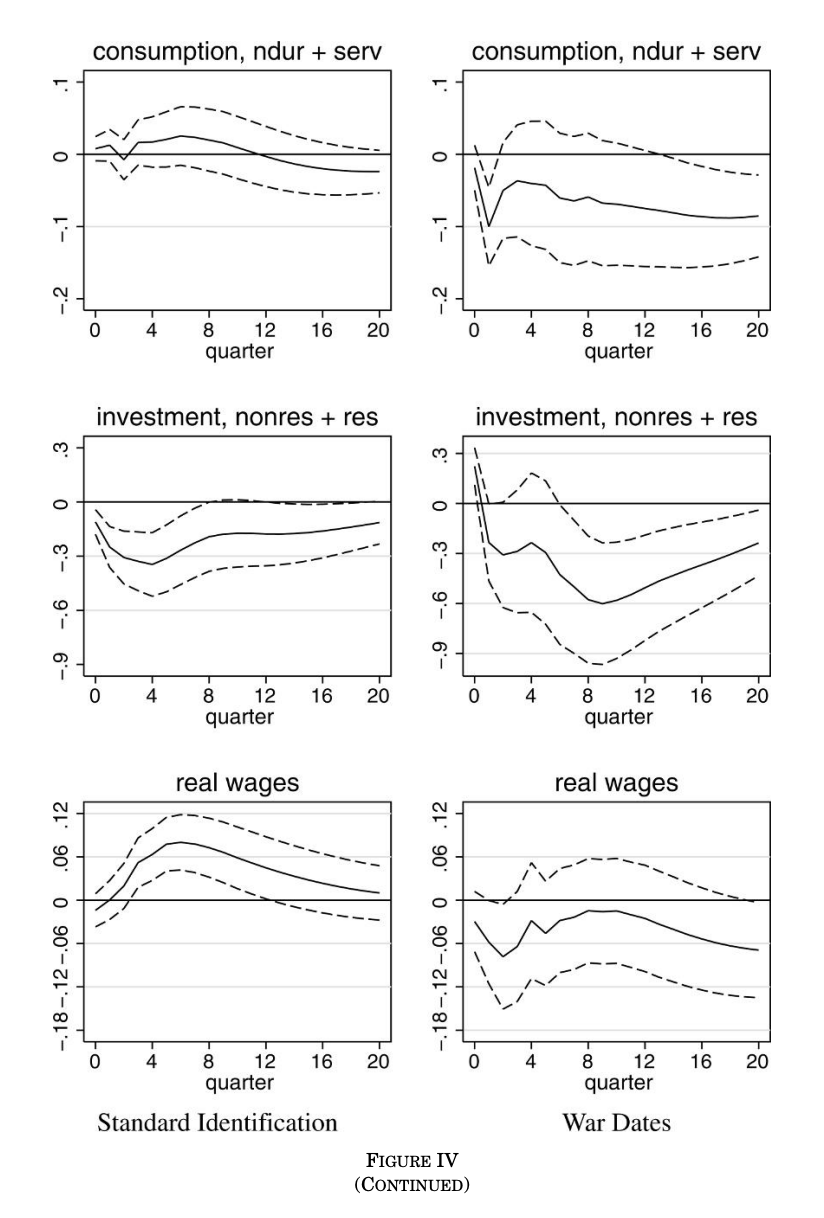
\includegraphics[scale=0.35]{FiguresTables/ramey_5}
\end{figure}
\end{frame}


\begin{frame}{Interpretation}
\begin{itemize}
\item Ramey argues that the difference has to do with timing
\item War dates recognize the release of information about future $G$. VAR does not.
\item Placebo: delay the war dates manually, and show you recover the IRFs by the VAR 
\end{itemize}
\end{frame}


\begin{frame}{The Power of Theory}
\begin{itemize}
\item VARs estimate an increase in consumption and real wages
\item War dates estimate a decrease in consumption and real wages
\item Literature spent too much time on this difference arguing it was informative on whether the world was Keynesian or not.
\item But you know better thanks to Woodford (2011): Keynesian models can predict $\uparrow C_t$ or $\downarrow C_t$ as a function of monetary policy!
\item The size of the multiplier, or its effects on consumption are not a testable implication of the NK model
\end{itemize}
\end{frame}


\begin{frame}{The Pros of using wars}
\begin{itemize}
\item Wars are used because they are more plausibly exogenous
\item Example. The American Recovery and Reinvestment Act enacted in the Obama years is clearly endogenous to the state (and future expected state) of the national US economy during the Great Financial Crisis.
\item Easier to argue that the US does not go to war because the economy is doing/expect to do poorly. WWII a great example.
\item Some episodes are also very large. Example: WWII also a great example for this. Even if other confounders, they should have small effects relative to $G$.
\end{itemize}
\end{frame}

\begin{frame}{External Validity}
\begin{itemize}
\item Now, even if we were to accept wars are exogenous, wars are special
\begin{itemize}
\item They trigger patriotism. So perhaps workers supply labor at constant wages, or firms more products at constant prices
\item in a way that would not happen in normal times
\item They come together with other policies that mediate the effects that would not take place. Examples: Wage and Price controls.
\item State planning more relevant. Inefficiencies?
\end{itemize}
\item Not obvious if the multiplier is too large or too small compared to normal periods
\item Barro thinks wars overestimate the multiplier. Hall thinks the contrary.
\end{itemize}
\end{frame}

\begin{frame}{Regional Shocks}
\begin{itemize}
\item A subsequent literature estimated the effects of changes in federal expenditures at the local level  on local economic conditions
\item Institutional background: When the federal US government increases military spending, it does so disproportionally in some states (a lot in CA, almost nothing in IL)
\item Variation advantage: In the time series, military spending moves very little after the Korean War.
\item 50 times more data at the state-level
\item Variation at the local level is larger.
\item Research design: Confounders that affect the national economy will be soaked by time fixed effects
\end{itemize}
\end{frame}

\begin{frame}{Nakamura Steinsson 2014}
\begin{figure}
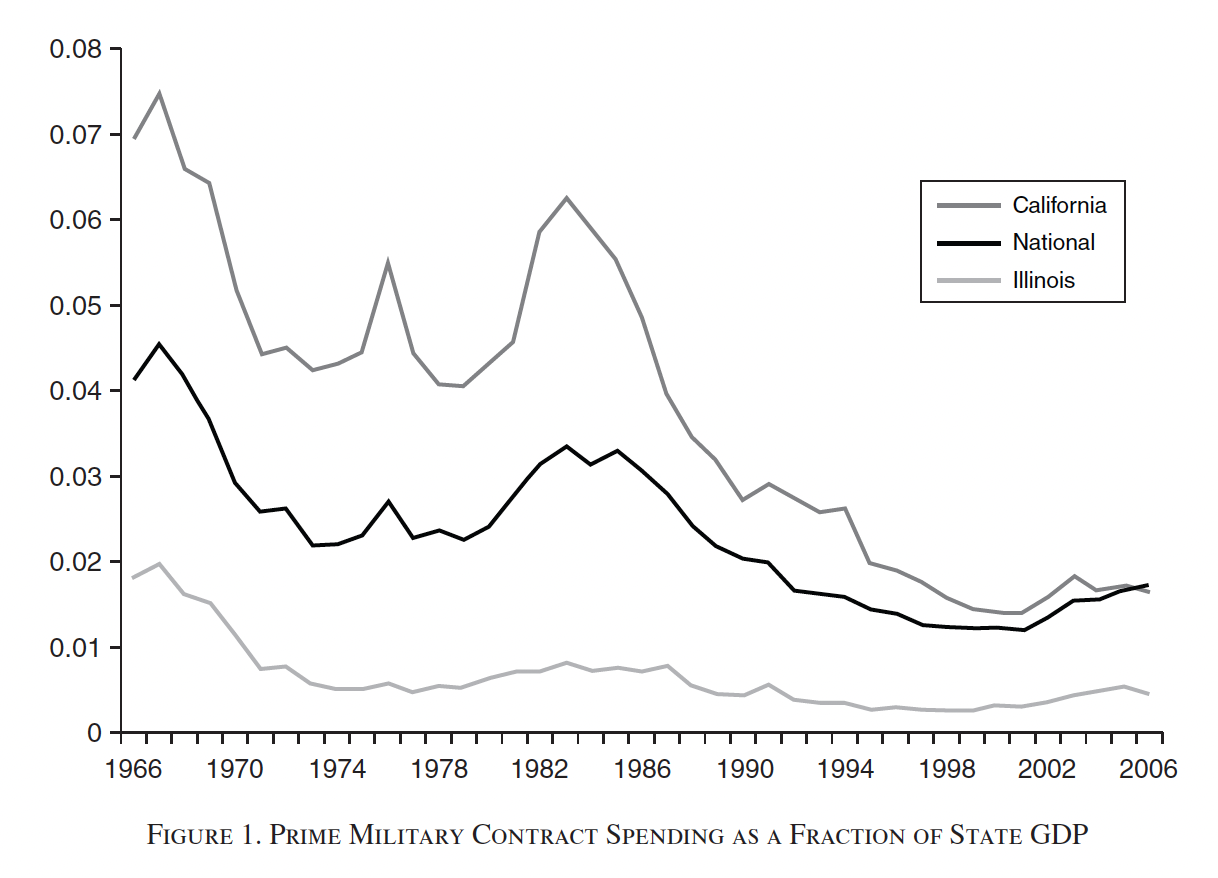
\includegraphics[scale=0.4]{FiguresTables/ns2014_1}
\end{figure}
\end{frame}


\begin{frame}{Specification}
\begin{align*}
\left(\frac{Y_{i,t} - Y_{i,t-2}}{Y_{i,t-2}}\right) = \alpha_i + \gamma_t + \beta	\left(\frac{G_{i,t} - G_{i,t-2}}{G_{i,t-2}}\right) + \epsilon_{it}
\end{align*}
\begin{itemize}
\item State fixed effects. State-specific trends
\item Time fixed effects. Controls for aggregate shocks.
\item Every variable measured in per-capita terms
\item Biannual regressions
\item $G_{it}$ potentially endogenous
\end{itemize}
\end{frame}

\begin{frame}{Instruments}
\begin{itemize}
\item Baseline Instrument. Sensitivity instrument
\begin{itemize}
\item National spending interacted with state dummy
\item How much $G_{it}$ increases when $G_t$ increases
\end{itemize}
\item Alternative instrument. Shift-Share/Bartik
\begin{itemize}
\item National spending (shifts) interacted with state average-spending in the first five years of the sample (shares)
\end{itemize}
\item Note that this weakens the identifying assumption in the literature. The US does not go to war because California is doing poorly relative to Illinois. It would be ok (for identification) if the US went to wars because the US economy is doing poorly.
\end{itemize}
\end{frame}

\begin{frame}{Results}
\begin{figure}
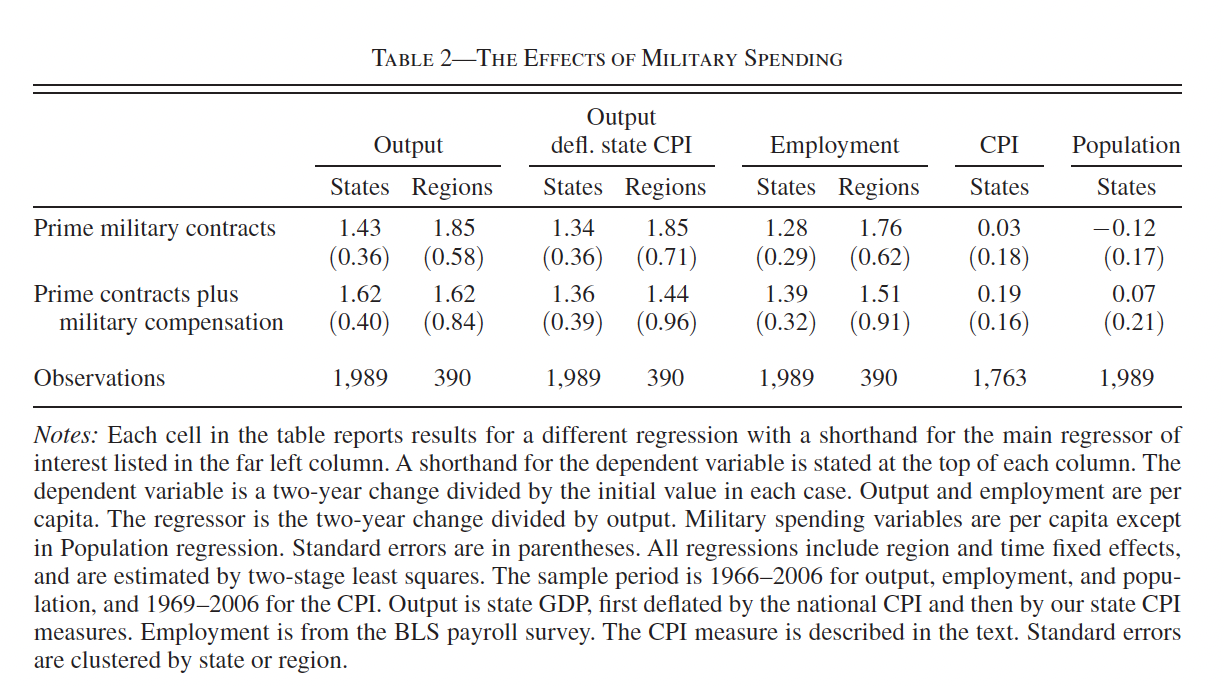
\includegraphics[scale=0.6]{FiguresTables/ns2014_2}
\end{figure}
\end{frame}

\begin{frame}{Regional vs. Aggregate Multipliers}
\begin{itemize}
\item Now, the object Nakamura and Steinsson are estimating is \textbf{not} the aggregate multiplier
\item Aggregate multiplier: What happens to US $GDP$ when US $G$ increases
\item NS2014: What happens to CA's GDP vs. IL's when $G$ increases in CA vs. IL.
\item Some advantages and disadvantages
\item Pros:
\begin{itemize}
\item Time fixed effects control for the reaction of the fed. Keeps nominal rates constant.
\item Argue that Keynesian models (not neoclassical models)  rationalize large cross-sectional multipliers
\item Causal inference: fixed effects and IVs purge bad variation
\end{itemize}
\item Cons:
\begin{itemize}
\item We are not directly learning about the object of interest
\item Many spillovers between treated and control states
\item Violations of SUTVA
\item Need to add a model to the causal inference exercise to infer the value of the aggregate multiplier
\end{itemize}
\end{itemize}
Will not go into details. Johannes and I teach a whole 2nd year class about these topics. 
\end{frame}




\end{document}




